\section{Desafio}

\begin{minipage}{\linewidth}
  \centering
  \begin{minipage}{0.45\linewidth}
    Dado o circuito da \textbf{Figura \ref{fig:CircuitoDesafio}}, identificar:
    \begin{itemize}
      \item Os componentes presentes;
      \item As funções de cada componente;
      \item A configuração de ligação dos componentes: série ou paralelo.
    \end{itemize}
  \end{minipage}
  \hspace{0.05\linewidth}
  \begin{minipage}{0.45\linewidth}
    \begin{figure}[H]
      \centering
      \caption{Circuito elétrico}
      \label{fig:CircuitoDesafio}
      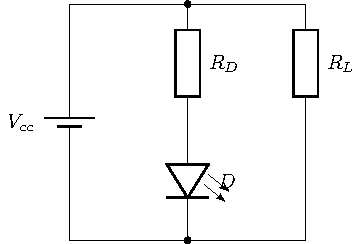
\includegraphics[scale=1.0]{fig-circuitoDesafio}
%
%      {\small Fonte: Próprio autor.}
    \end{figure}
  \end{minipage}
\end{minipage}
